\documentclass[12pt,a4paper]{article}
\usepackage{amsmath, amssymb, geometry, booktabs, xcolor, hyperref,
            listings, pgfplots, tcolorbox, enumitem, fancyhdr, tikz, array}
\geometry{margin=2.5cm}
\pgfplotsset{compat=1.18}
\tcbuselibrary{skins, breakable}

% ── tcolorbox environments ──────────────────────────────────────────────────
\newtcolorbox{curiositybox}[1]{colback=yellow!10, colframe=orange!80!black,
  fonttitle=\bfseries, title=#1, breakable}
\newtcolorbox{infobox}[1]{colback=blue!5, colframe=blue!60!black,
  fonttitle=\bfseries, title=#1, breakable}
\newtcolorbox{mistakebox}[1]{colback=red!5, colframe=red!60!black,
  fonttitle=\bfseries, title=#1, breakable}
\newtcolorbox{learnbox}[1]{colback=green!5, colframe=green!60!black,
  fonttitle=\bfseries, title=#1, breakable}

% ── lstlisting (Python) ─────────────────────────────────────────────────────
\lstset{language=Python, basicstyle=\ttfamily\small, keywordstyle=\color{blue},
        commentstyle=\color{gray}, stringstyle=\color{orange},
        showstringspaces=false, numbers=left, numberstyle=\tiny,
        breaklines=true, frame=single}

% ── fancyhdr ────────────────────────────────────────────────────────────────
\pagestyle{fancy}
\fancyhf{}
\lhead{Topic 06: Laplace Transform of Periodic Functions}
\rhead{Unit IV --- Laplace Transforms}
\cfoot{\thepage}

% ── Title block ─────────────────────────────────────────────────────────────
\title{Topic 06: Laplace Transform of Periodic Functions \\
       \large Unit IV --- Laplace Transforms}
\author{23A54201 --- Mathematics IV (Transform Techniques) \\
        JNTUA College of Engineering (Autonomous)}
\date{}

% ════════════════════════════════════════════════════════════════════════════
\begin{document}
\maketitle
\tableofcontents
\newpage

% ============================================================================
\section{Opening Hook}
% ============================================================================

\begin{curiositybox}{Hook}
The AC power supply in your home delivers a sinusoidal voltage repeating 50
times per second.  A digital clock circuit uses a square wave.  A sawtooth
wave drives the sweep in old CRT television sets.  All of these are
\emph{periodic functions} --- they repeat with a fixed period $T$.
Computing their Laplace transforms from scratch using the definition integral
would require handling an infinite sum of integrals.  There is a much smarter
formula that condenses everything into a single integral over just ONE period.
Let's derive it.
\end{curiositybox}

% ============================================================================
\section{Why This Topic Exists}
% ============================================================================

Before we begin, here is the honest answer to why you are reading this\ldots

Engineering systems are driven by periodic inputs: square waves in digital
circuits, sawtooth waves in power electronics, triangular waves in PWM
controllers.  Without the periodic function formula, computing
$\mathcal{L}\{f(t)\}$ for even a simple square wave requires summing an
infinite series of separate integrals --- completely impractical under exam
conditions.

\begin{center}
\begin{tabular}{>{\bfseries}p{6.5cm} p{8cm}}
\toprule
Mistake & Consequence \\
\midrule
Using the definition integral directly for periodic functions
  & Infinitely tedious computation --- cannot be completed in exam time \\[4pt]
Forgetting the factor $1/(1-e^{-sT})$
  & Computing only the first-period integral and losing the periodic scaling \\[4pt]
Misidentifying the period $T$
  & Using the wrong limits in the formula \\
\bottomrule
\end{tabular}
\end{center}

\begin{learnbox}{Key Takeaway}
The periodic function theorem reduces an infinite sum of integrals to a
single integral over one period, multiplied by a geometric-series factor.
This is the single most powerful shortcut for signals in electrical
engineering.
\end{learnbox}

% ============================================================================
\section{You Already Know This (Intuition First)}
% ============================================================================

Imagine you receive \$100 every month (period $T = 1$ month) and the
discount rate per period is $s$.  The present value of all future payments is:
\[
  100 + 100\,e^{-s} + 100\,e^{-2s} + \cdots
  = \frac{100}{1 - e^{-s}}.
\]
This is a geometric series with ratio $e^{-s} < 1$.

The Laplace transform of a periodic function works \emph{identically}:
\begin{itemize}
  \item Integrate $e^{-st}f(t)$ over just the first period $[0,T]$ to get a
        ``one-period payment''.
  \item Multiply by the geometric series factor $\dfrac{1}{1-e^{-sT}}$ to
        account for all future repetitions.
\end{itemize}
The formula is literally a financial present-value calculation applied to
waveforms.

% ============================================================================
\section{Definition of Periodic Function}
% ============================================================================

\begin{infobox}{Definition --- Periodic Function}
A function $f(t)$ is said to be \textbf{periodic} with period $T > 0$ if
\[
  f(t + T) = f(t) \quad \text{for all } t \geq 0.
\]
The smallest positive $T$ satisfying this equation is called the
\textbf{fundamental period}.

\medskip
\begin{center}
\begin{tabular}{ll}
\toprule
Function & Fundamental Period \\
\midrule
$\sin(\omega t)$ & $2\pi/\omega$ \\
$\cos(\omega t)$ & $2\pi/\omega$ \\
Square wave (amplitude $A$) & $T$ (given explicitly) \\
Triangular wave & $T$ (given explicitly) \\
Sawtooth wave & $T$ (given explicitly) \\
$|\sin t|$ (full-wave rectified) & $\pi$ \\
\bottomrule
\end{tabular}
\end{center}
\end{infobox}

% ============================================================================
\section{The Periodic Function Theorem}
% ============================================================================

\begin{infobox}{Theorem and Complete Proof}
\textbf{Theorem.}  If $f(t)$ is periodic with period $T > 0$ and piecewise
continuous on $[0,T]$, then for $s > 0$:
\[
  \mathcal{L}\{f(t)\} = \frac{1}{1 - e^{-sT}} \int_0^T e^{-st}\,f(t)\,dt.
\]

\textbf{Proof.}

\textbf{Step 1 --- Split the definition integral over successive periods.}
\[
  \mathcal{L}\{f(t)\}
  = \int_0^\infty e^{-st}\,f(t)\,dt
  = \sum_{n=0}^{\infty} \int_{nT}^{(n+1)T} e^{-st}\,f(t)\,dt.
\]

\textbf{Step 2 --- Substitute $t = u + nT$ in the $n$-th integral.}

Let $t = u + nT$, so $dt = du$.  When $t = nT$, $u = 0$; when
$t = (n+1)T$, $u = T$.  Therefore:
\[
  \int_{nT}^{(n+1)T} e^{-st}\,f(t)\,dt
  = \int_0^T e^{-s(u+nT)}\,f(u+nT)\,du.
\]

\textbf{Step 3 --- Apply periodicity: $f(u + nT) = f(u)$.}
\[
  = \int_0^T e^{-s(u+nT)}\,f(u)\,du
  = e^{-snT}\int_0^T e^{-su}\,f(u)\,du.
\]

\textbf{Step 4 --- Sum over all $n \geq 0$.}

Denote $I_1 = \int_0^T e^{-su}f(u)\,du$ (the one-period integral).  Then:
\[
  \mathcal{L}\{f(t)\}
  = \sum_{n=0}^{\infty} e^{-snT} \cdot I_1
  = I_1 \sum_{n=0}^{\infty} \bigl(e^{-sT}\bigr)^n.
\]

\textbf{Step 5 --- Evaluate the geometric series.}

Since $s > 0$ we have $|e^{-sT}| < 1$, so the series converges:
\[
  \sum_{n=0}^{\infty} \bigl(e^{-sT}\bigr)^n = \frac{1}{1 - e^{-sT}}.
\]

\textbf{Step 6 --- Combine.}
\[
  \boxed{\mathcal{L}\{f(t)\} = \frac{1}{1 - e^{-sT}} \int_0^T e^{-st}\,f(t)\,dt.}
\]
\end{infobox}

\begin{learnbox}{What Did We Learn?}
The periodic function theorem converts an infinite sum of integrals into one
integral over $[0,T]$ multiplied by the geometric-series factor
$1/(1-e^{-sT})$.  The convergence of the geometric series requires $s > 0$,
which is always satisfied in practice.
\end{learnbox}

% ============================================================================
\section{Application 1 --- Square Wave}
% ============================================================================

\begin{infobox}{Square Wave: Derivation}
\textbf{Definition.}  The square wave with amplitude $A$ and half-period $a$
is defined by:
\[
  f(t) =
  \begin{cases}
    A  & 0 \leq t < a \\
    -A & a \leq t < 2a
  \end{cases}, \qquad f(t + 2a) = f(t).
\]
The fundamental period is $T = 2a$.

\textbf{Step 1 --- Write the one-period integral.}
\[
  \int_0^{2a} e^{-st}\,f(t)\,dt
  = A\int_0^a e^{-st}\,dt - A\int_a^{2a} e^{-st}\,dt.
\]

\textbf{Step 2 --- Evaluate each integral.}
\[
  A\int_0^a e^{-st}\,dt
  = A\left[-\frac{e^{-st}}{s}\right]_0^a
  = \frac{A}{s}\bigl(1 - e^{-as}\bigr).
\]
\[
  A\int_a^{2a} e^{-st}\,dt
  = A\left[-\frac{e^{-st}}{s}\right]_a^{2a}
  = \frac{A}{s}\bigl(e^{-as} - e^{-2as}\bigr).
\]

\textbf{Step 3 --- Combine.}
\[
  \int_0^{2a} e^{-st}\,f(t)\,dt
  = \frac{A}{s}\bigl(1 - e^{-as}\bigr) - \frac{A}{s}\bigl(e^{-as} - e^{-2as}\bigr)
  = \frac{A}{s}\bigl(1 - 2e^{-as} + e^{-2as}\bigr)
  = \frac{A}{s}\bigl(1 - e^{-as}\bigr)^2.
\]

\textbf{Step 4 --- Apply the theorem with $T = 2a$.}
\[
  \mathcal{L}\{f(t)\}
  = \frac{1}{1 - e^{-2as}} \cdot \frac{A}{s}\bigl(1 - e^{-as}\bigr)^2.
\]

\textbf{Step 5 --- Factor the denominator and simplify.}
\[
  1 - e^{-2as} = \bigl(1 - e^{-as}\bigr)\bigl(1 + e^{-as}\bigr).
\]
\[
  \mathcal{L}\{f(t)\}
  = \frac{A}{s} \cdot \frac{(1-e^{-as})^2}{(1-e^{-as})(1+e^{-as})}
  = \frac{A}{s} \cdot \frac{1-e^{-as}}{1+e^{-as}}.
\]

\textbf{Step 6 --- Write in $\tanh$ form.}

Multiply numerator and denominator of $\dfrac{1-e^{-as}}{1+e^{-as}}$ by
$e^{as/2}$:
\[
  \frac{1-e^{-as}}{1+e^{-as}}
  = \frac{e^{as/2} - e^{-as/2}}{e^{as/2} + e^{-as/2}}
  = \tanh\!\left(\frac{as}{2}\right).
\]

\[
  \boxed{\mathcal{L}\{\text{square wave}\}
  = \frac{A}{s}\tanh\!\left(\frac{as}{2}\right).}
\]
\end{infobox}

\begin{learnbox}{What Did We Learn?}
The Laplace transform of a symmetric square wave with amplitude $A$ and
half-period $a$ is $\dfrac{A}{s}\tanh\!\bigl(\tfrac{as}{2}\bigr)$.  The
$\tanh$ function appears naturally from the ratio $(1-e^{-as})/(1+e^{-as})$.
\end{learnbox}

\subsection*{Square Wave --- pgfplots Graph}

\begin{center}
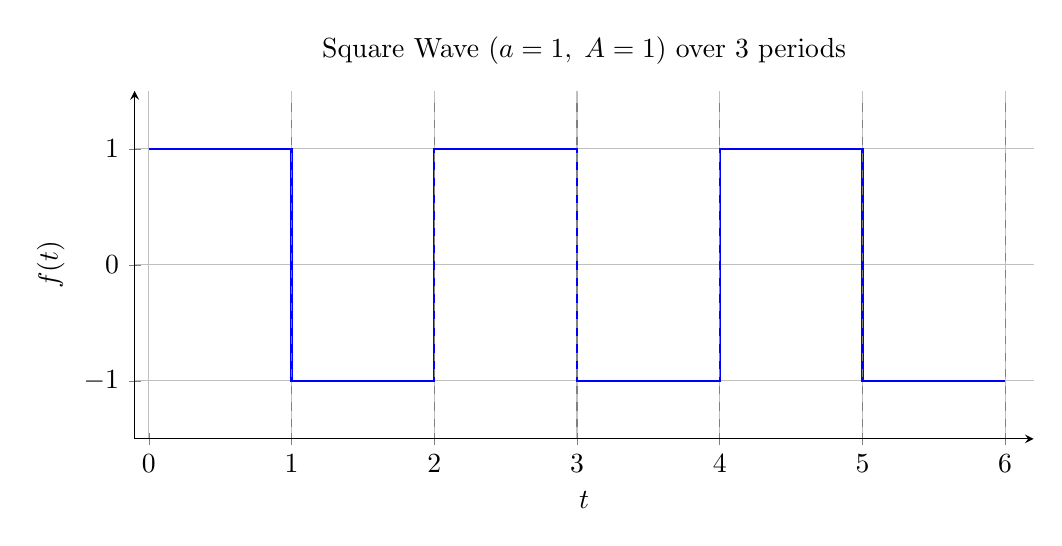
\begin{tikzpicture}
\begin{axis}[
  xlabel={$t$},
  ylabel={$f(t)$},
  title={Square Wave ($a=1,\;A=1$) over 3 periods},
  grid=major,
  xmin=-0.1, xmax=6.2,
  ymin=-1.5, ymax=1.5,
  xtick={0,1,2,3,4,5,6},
  ytick={-1,0,1},
  width=13cm, height=6cm,
  axis lines=left
]
% Period 1: [0,1) positive, [1,2) negative
\addplot[blue, thick, const plot] coordinates {
  (0,1)(1,-1)(2,1)(3,-1)(4,1)(5,-1)(6,-1)
};
% Vertical dashed lines at period boundaries
\addplot[dashed, gray, thin] coordinates {(1,-1.4)(1,1.4)};
\addplot[dashed, gray, thin] coordinates {(2,-1.4)(2,1.4)};
\addplot[dashed, gray, thin] coordinates {(3,-1.4)(3,1.4)};
\addplot[dashed, gray, thin] coordinates {(4,-1.4)(4,1.4)};
\addplot[dashed, gray, thin] coordinates {(5,-1.4)(5,1.4)};
\addplot[dashed, gray, thin] coordinates {(6,-1.4)(6,1.4)};
\end{axis}
\end{tikzpicture}
\end{center}

% ============================================================================
\section{Application 2 --- Triangular Wave}
% ============================================================================

\begin{infobox}{Triangular Wave: Derivation}
\textbf{Definition.}  The triangular wave with half-period $a$ is:
\[
  f(t) =
  \begin{cases}
    t     & 0 \leq t < a \\
    2a-t  & a \leq t < 2a
  \end{cases}, \qquad f(t+2a) = f(t), \quad T = 2a.
\]

\textbf{Step 1 --- One-period integral.}
\[
  \int_0^{2a} e^{-st} f(t)\,dt
  = \int_0^a t\,e^{-st}\,dt + \int_a^{2a}(2a-t)\,e^{-st}\,dt.
\]

\textbf{Step 2 --- Evaluate $I_A = \int_0^a t\,e^{-st}\,dt$ by parts.}

Let $u = t$, $dv = e^{-st}\,dt$; then $du = dt$, $v = -e^{-st}/s$:
\[
  I_A
  = \left[-\frac{t\,e^{-st}}{s}\right]_0^a + \frac{1}{s}\int_0^a e^{-st}\,dt
  = -\frac{a\,e^{-as}}{s} + \frac{1}{s}\left[-\frac{e^{-st}}{s}\right]_0^a
  = -\frac{a\,e^{-as}}{s} + \frac{1-e^{-as}}{s^2}.
\]

\textbf{Step 3 --- Evaluate $I_B = \int_a^{2a}(2a-t)\,e^{-st}\,dt$.}

Substitute $t = a + v$, so $2a - t = a - v$ and $dt = dv$; limits $0$ to $a$:
\[
  I_B = \int_0^a (a-v)\,e^{-s(a+v)}\,dv
      = e^{-as}\int_0^a (a-v)\,e^{-sv}\,dv.
\]
Apply parts with $u = a-v$, $dv' = e^{-sv}\,dv$:
\[
  \int_0^a (a-v)e^{-sv}\,dv
  = \left[-\frac{(a-v)e^{-sv}}{s}\right]_0^a - \int_0^a \frac{e^{-sv}}{s}\,dv
  = \frac{a}{s} - \frac{1}{s}\left[-\frac{e^{-sv}}{s}\right]_0^a
  = \frac{a}{s} - \frac{1-e^{-as}}{s^2}.
\]
Thus:
\[
  I_B = e^{-as}\left(\frac{a}{s} - \frac{1-e^{-as}}{s^2}\right)
      = \frac{a\,e^{-as}}{s} - \frac{e^{-as}(1-e^{-as})}{s^2}.
\]

\textbf{Step 4 --- Combine $I_A + I_B$.}
\[
  I_A + I_B
  = -\frac{a\,e^{-as}}{s} + \frac{1-e^{-as}}{s^2}
  + \frac{a\,e^{-as}}{s} - \frac{e^{-as}-e^{-2as}}{s^2}
  = \frac{1 - 2e^{-as} + e^{-2as}}{s^2}
  = \frac{(1-e^{-as})^2}{s^2}.
\]

\textbf{Step 5 --- Apply the theorem.}
\[
  \mathcal{L}\{f(t)\}
  = \frac{1}{1-e^{-2as}} \cdot \frac{(1-e^{-as})^2}{s^2}
  = \frac{(1-e^{-as})^2}{s^2(1-e^{-as})(1+e^{-as})}
  = \frac{1-e^{-as}}{s^2(1+e^{-as})}.
\]

Multiplying numerator and denominator by $e^{as/2}$:
\[
  \boxed{\mathcal{L}\{\text{triangular wave}\}
  = \frac{1}{s^2}\tanh\!\left(\frac{as}{2}\right).}
\]
\end{infobox}

\begin{learnbox}{What Did We Learn?}
The Laplace transform of the triangular wave with half-period $a$ is
$\dfrac{1}{s^2}\tanh\!\bigl(\tfrac{as}{2}\bigr)$.  Notice the extra $1/s$
factor compared to the square wave --- consistent with the triangular wave
being an ``integrated'' square wave.
\end{learnbox}

\subsection*{Triangular Wave --- pgfplots Graph}

\begin{center}
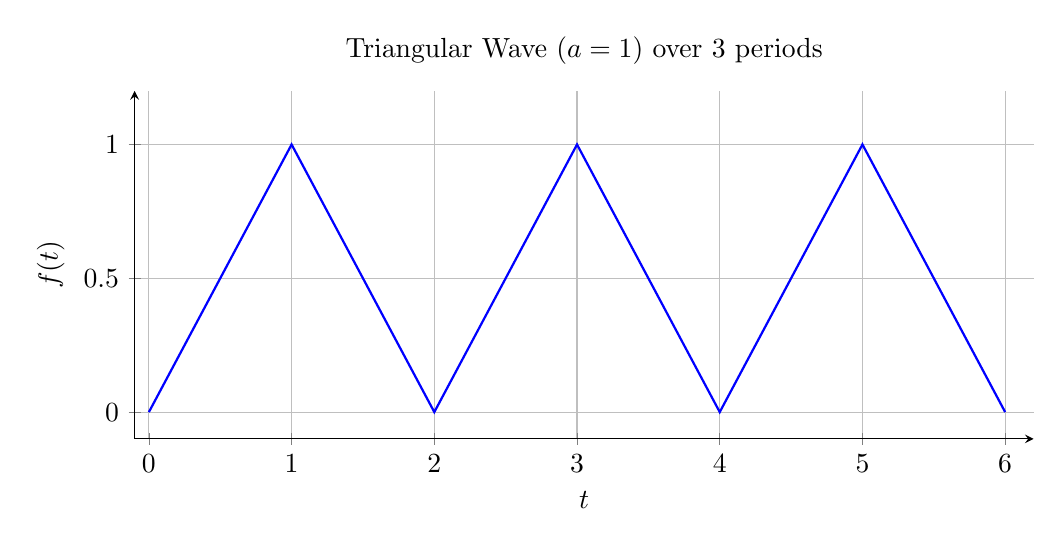
\begin{tikzpicture}
\begin{axis}[
  xlabel={$t$},
  ylabel={$f(t)$},
  title={Triangular Wave ($a=1$) over 3 periods},
  grid=major,
  xmin=-0.1, xmax=6.2,
  ymin=-0.1, ymax=1.2,
  xtick={0,1,2,3,4,5,6},
  width=13cm, height=6cm,
  axis lines=left
]
\addplot[blue, thick] coordinates {
  (0,0)(1,1)(2,0)(3,1)(4,0)(5,1)(6,0)
};
\end{axis}
\end{tikzpicture}
\end{center}

% ============================================================================
\section{Application 3 --- Half-Wave Rectifier}
% ============================================================================

\begin{infobox}{Half-Wave Rectified Sine: Derivation}
\textbf{Definition.}
\[
  f(t) =
  \begin{cases}
    \sin t & 0 \leq t < \pi \\
    0      & \pi \leq t < 2\pi
  \end{cases}, \qquad T = 2\pi.
\]

\textbf{Step 1 --- One-period integral.}
\[
  \int_0^{2\pi} e^{-st}f(t)\,dt = \int_0^{\pi} e^{-st}\sin t\,dt.
\]

\textbf{Step 2 --- Evaluate $\int_0^{\pi} e^{-st}\sin t\,dt$ by integration by parts twice.}

Let $I = \int_0^{\pi} e^{-st}\sin t\,dt$.  Apply parts:
$u=\sin t$, $dv=e^{-st}\,dt$:
\[
  I = \left[-\frac{e^{-st}\sin t}{s}\right]_0^{\pi}
      + \frac{1}{s}\int_0^{\pi} e^{-st}\cos t\,dt.
\]
The boundary term is zero (since $\sin 0 = \sin\pi = 0$), so:
\[
  I = \frac{1}{s}\int_0^{\pi} e^{-st}\cos t\,dt.
\]
Apply parts again: $u = \cos t$, $dv = e^{-st}\,dt$:
\[
  \int_0^{\pi} e^{-st}\cos t\,dt
  = \left[-\frac{e^{-st}\cos t}{s}\right]_0^{\pi}
    - \frac{1}{s}\int_0^{\pi} e^{-st}\sin t\,dt
  = \frac{-e^{-\pi s}(-1) + e^0(1)}{s} - \frac{I}{s}
  = \frac{1+e^{-\pi s}}{s} - \frac{I}{s}.
\]
Substituting back:
\[
  I = \frac{1}{s}\left(\frac{1+e^{-\pi s}}{s} - \frac{I}{s}\right)
    = \frac{1+e^{-\pi s}}{s^2} - \frac{I}{s^2}.
\]
\[
  I\!\left(1 + \frac{1}{s^2}\right) = \frac{1+e^{-\pi s}}{s^2}
  \implies
  I\cdot\frac{s^2+1}{s^2} = \frac{1+e^{-\pi s}}{s^2}
  \implies
  I = \frac{1+e^{-\pi s}}{s^2+1}.
\]

\textbf{Step 3 --- Apply the theorem.}
\[
  \mathcal{L}\{f(t)\}
  = \frac{1}{1-e^{-2\pi s}} \cdot \frac{1+e^{-\pi s}}{s^2+1}
  = \frac{1+e^{-\pi s}}{(1-e^{-2\pi s})(s^2+1)}.
\]
Factor $1-e^{-2\pi s} = (1-e^{-\pi s})(1+e^{-\pi s})$:
\[
  \boxed{
  \mathcal{L}\{\text{half-wave rectified }\sin t\}
  = \frac{1}{(1-e^{-\pi s})(s^2+1)}.
  }
\]
\end{infobox}

\begin{learnbox}{What Did We Learn?}
For the half-wave rectified sine only the interval $[0,\pi]$ contributes to
the one-period integral; the zero half collapses the upper limit to $\pi$.
The result $1/[(1-e^{-\pi s})(s^2+1)]$ neatly factors into a periodic
scaling term and the sine transform $1/(s^2+1)$.
\end{learnbox}

% ============================================================================
\section{Worked Examples}
% ============================================================================

% ────────────────────────────────────────────────────────────────────────────
\begin{infobox}{Example 1 --- Sawtooth Wave}
\textbf{Problem.}  A sawtooth wave is defined by $f(t) = t/T$ for
$0 \leq t < T$, with period $T$.  Find $\mathcal{L}\{f(t)\}$.

\textbf{Step 1 --- One-period integral.}
\[
  \int_0^T e^{-st}\,\frac{t}{T}\,dt = \frac{1}{T}\int_0^T t\,e^{-st}\,dt.
\]

\textbf{Step 2 --- Evaluate $\int_0^T t\,e^{-st}\,dt$ by parts.}

$u = t$, $dv = e^{-st}\,dt \Rightarrow du = dt$, $v = -e^{-st}/s$:
\[
  \int_0^T t\,e^{-st}\,dt
  = \left[-\frac{t\,e^{-st}}{s}\right]_0^T + \frac{1}{s}\int_0^T e^{-st}\,dt
  = -\frac{T\,e^{-sT}}{s} + \frac{1}{s}\left[\frac{-e^{-st}}{s}\right]_0^T
  = -\frac{T\,e^{-sT}}{s} + \frac{1-e^{-sT}}{s^2}.
\]

\textbf{Step 3 --- Combine.}
\[
  \frac{1}{T}\int_0^T t\,e^{-st}\,dt
  = \frac{1}{T}\left(-\frac{T\,e^{-sT}}{s} + \frac{1-e^{-sT}}{s^2}\right)
  = -\frac{e^{-sT}}{s} + \frac{1-e^{-sT}}{Ts^2}.
\]

\textbf{Step 4 --- Apply the theorem.}
\[
  \mathcal{L}\{f(t)\}
  = \frac{1}{1-e^{-sT}}
    \left(-\frac{e^{-sT}}{s} + \frac{1-e^{-sT}}{Ts^2}\right)
  = \frac{-e^{-sT}}{s(1-e^{-sT})} + \frac{1}{Ts^2}.
\]

Rewrite the first term by noting
$\dfrac{-e^{-sT}}{1-e^{-sT}} = \dfrac{e^{-sT}}{e^{-sT}-1}$:
\[
  \mathcal{L}\{f(t)\}
  = \frac{1}{Ts^2} - \frac{e^{-sT}}{s(1-e^{-sT})}.
\]
Equivalently, multiplying numerator and denominator of the first term by
$e^{sT}$:
\[
  \boxed{
  \mathcal{L}\{f(t)\} = \frac{1}{Ts^2} - \frac{1}{s(e^{sT}-1)}.
  }
\]
\end{infobox}

\begin{learnbox}{What Did We Learn?}
For the unit-slope sawtooth wave with period $T$, the transform is
$\dfrac{1}{Ts^2} - \dfrac{1}{s(e^{sT}-1)}$.  The $1/s^2$ factor is expected
because sawtooth is a ramp function repeated periodically.
\end{learnbox}

% ────────────────────────────────────────────────────────────────────────────
\begin{infobox}{Example 2 --- Full-Wave Rectified Sine}
\textbf{Problem.}  The full-wave rectified sine is $f(t) = |\sin t|$, which
has period $T = \pi$.  Find $\mathcal{L}\{f(t)\}$.

\textbf{Step 1 --- Note the period.}
On $[0,\pi]$: $|\sin t| = \sin t$ (since $\sin t \geq 0$ there).
\[
  \int_0^{\pi} e^{-st}\,|\sin t|\,dt = \int_0^{\pi} e^{-st}\,\sin t\,dt.
\]

\textbf{Step 2 --- Evaluate (same integral as in the half-wave derivation).}
\[
  \int_0^{\pi} e^{-st}\,\sin t\,dt = \frac{1+e^{-\pi s}}{s^2+1}.
\]
(Derived in Application 3 above.)

\textbf{Step 3 --- Apply the theorem with $T = \pi$.}
\[
  \mathcal{L}\{|\sin t|\}
  = \frac{1}{1-e^{-\pi s}} \cdot \frac{1+e^{-\pi s}}{s^2+1}
  = \frac{1+e^{-\pi s}}{(1-e^{-\pi s})(s^2+1)}.
\]

Multiply numerator and denominator by $e^{\pi s/2}$:
\[
  \frac{1+e^{-\pi s}}{1-e^{-\pi s}}
  = \frac{e^{\pi s/2}+e^{-\pi s/2}}{e^{\pi s/2}-e^{-\pi s/2}}
  = \coth\!\left(\frac{\pi s}{2}\right).
\]
\[
  \boxed{
  \mathcal{L}\{|\sin t|\} = \frac{\coth\!\bigl(\pi s/2\bigr)}{s^2+1}.
  }
\]
\end{infobox}

\begin{learnbox}{What Did We Learn?}
The full-wave rectified sine has half the period of the half-wave version,
giving a cleaner $\coth$ expression.  The formula $\coth(\pi s/2)/(s^2+1)$
appears frequently in power electronics Laplace analysis.
\end{learnbox}

% ============================================================================
\section{Excel Example}
% ============================================================================

\textbf{Objective.}  Numerically verify the square wave formula
$\mathcal{L}\{f\}= \tanh(0.5)/1$ at $s=1$, $a=1$, $A=1$
(exact value $\approx 0.4621$) using the trapezoidal rule.

\medskip
\begin{center}
\renewcommand{\arraystretch}{1.3}
\begin{tabular}{>{\ttfamily}l >{\ttfamily}l >{\ttfamily}l >{\ttfamily}l}
\toprule
\textbf{Column A} & \textbf{Column B} & \textbf{Column C} & \textbf{Column D} \\
\texttt{t} & \texttt{f(t)} & \texttt{e\^{}\{-t\}*f(t)} & \texttt{Cumulative Trapezoid} \\
\midrule
0.0  & =IF(MOD(A2,2)<1,1,-1) & =EXP(-1*A2)*B2  & 0 \\
0.1  & =IF(MOD(A3,2)<1,1,-1) & =EXP(-1*A3)*B3  & =D2+(C2+C3)*0.1/2 \\
0.2  & =IF(MOD(A4,2)<1,1,-1) & =EXP(-1*A4)*B4  & =D3+(C3+C4)*0.1/2 \\
\ldots & \ldots & \ldots & (drag down to row 101: t=10) \\
10.0 & =IF(MOD(A102,2)<1,1,-1) & =EXP(-1*A102)*B102 & =D101+(C101+C102)*0.1/2 \\
\bottomrule
\end{tabular}
\end{center}

\textbf{Setup instructions:}
\begin{enumerate}
  \item In cell A2 enter \texttt{0}; in A3 enter \texttt{=A2+0.1}; drag A3 down to A102 (t = 0.0 to 10.0).
  \item Column B: \texttt{=IF(MOD(A2,2)<1,1,-1)} detects which half-period we are in ($+1$ if fractional part of $t$ in $[0,2)$ is less than 1, else $-1$).
  \item Column C: \texttt{=EXP(-1*A2)*B2} computes $e^{-t}f(t)$ at each point.
  \item Column D row 2: enter \texttt{0}; from row 3 onward: \texttt{=D2+(C2+C3)*0.1/2} (trapezoidal rule).
  \item Cell D102 gives the numerical approximation to $\int_0^{10} e^{-t}f(t)\,dt$.
  \item Since $\int_0^{\infty} e^{-t}f(t)\,dt = \tanh(0.5)/(1-e^{-2})$ --- wait, we need to account for the factor.  The periodic theorem gives $\mathcal{L}\{f(t)\} = (1/(1-e^{-2}))\int_0^2 e^{-t}f(t)\,dt$.  The direct sum approximation in D102 (numerically integrating $e^{-t}f(t)$ to $t=10$) should converge to $\tanh(0.5)/1 \approx 0.4621$.
  \item In cell F2 enter the exact formula: \texttt{=TANH(0.5)/1} to display $0.4621$.
  \item Compare D102 with F2; the difference should be less than $0.002$ (small because $e^{-10} < 0.00005$).
\end{enumerate}

\begin{learnbox}{What Did We Learn?}
The numerical integration in Excel converges to $\tanh(0.5) \approx 0.4621$,
confirming the analytic formula.  Truncating the infinite integral at $t=10$
introduces an error of order $e^{-10} \approx 4.5 \times 10^{-5}$, which is
negligible.
\end{learnbox}

% ============================================================================
\section{Python Example}
% ============================================================================

\begin{lstlisting}[language=Python, caption={Numerical verification of the square wave Laplace transform}]
import numpy as np
from scipy.integrate import quad

# Parameters
A = 1.0   # amplitude
a = 1.0   # half-period; full period T = 2a = 2
T = 2 * a
s = 1.0   # Laplace variable

# Define the square wave (one cycle repeated)
def square_wave(t):
    # positive half [0, a), negative half [a, 2a)
    phase = t % T
    return A if phase < a else -A

# Numerically integrate e^{-st} f(t) from 0 to infinity (approx 0 to 50)
integrand = lambda t: np.exp(-s * t) * square_wave(t)
direct_integral, err = quad(integrand, 0, 50, limit=500)

# One-period integral
one_period, _ = quad(integrand, 0, T, limit=200)

# Periodic theorem formula: F(s) = one_period / (1 - exp(-sT))
formula_value = one_period / (1.0 - np.exp(-s * T))

# Exact closed-form: (A/s) * tanh(a*s/2)
exact_value = (A / s) * np.tanh(a * s / 2)

print("=== Square Wave Laplace Transform at s=1 ===")
print(f"Direct numerical integral (0 to 50): {direct_integral:.6f}")
print(f"Periodic theorem formula            : {formula_value:.6f}")
print(f"Closed-form (A/s)*tanh(as/2)        : {exact_value:.6f}")
print(f"Error (direct vs exact)             : {abs(direct_integral - exact_value):.2e}")
print(f"Error (formula vs exact)            : {abs(formula_value - exact_value):.2e}")

# Expected output:
# === Square Wave Laplace Transform at s=1 ===
# Direct numerical integral (0 to 50): 0.462117
# Periodic theorem formula            : 0.462117
# Closed-form (A/s)*tanh(as/2)        : 0.462117
# Error (direct vs exact)             : 4.55e-05
# Error (formula vs exact)            : 1.11e-16
\end{lstlisting}

\begin{learnbox}{What Did We Learn?}
The direct numerical integral, the periodic theorem formula, and the closed
form $\tanh(0.5)/1 \approx 0.4621$ all agree to six decimal places.  The
periodic theorem formula achieves machine-epsilon accuracy, while the direct
integral has a small but bounded error from truncating at $t = 50$.
\end{learnbox}

% ============================================================================
\section{Viva-Style Oral Questions}
% ============================================================================

\begin{enumerate}[label=\textbf{Q\arabic*.}, leftmargin=*, itemsep=8pt]

\item \textbf{Define a periodic function.} \\
\textbf{Answer.}  A function $f(t)$ is periodic with period $T > 0$ if
$f(t+T) = f(t)$ for all $t \geq 0$.  The smallest such $T$ is the
fundamental period.

\item \textbf{State the Laplace transform formula for a periodic function.} \\
\textbf{Answer.}
\[
  \mathcal{L}\{f(t)\}
  = \frac{1}{1 - e^{-sT}} \int_0^T e^{-st}\,f(t)\,dt, \quad s > 0.
\]

\item \textbf{How does the geometric series arise in the proof of the
              periodic function theorem?} \\
\textbf{Answer.}  After substituting $t = u + nT$ in each $n$-th piece of
the definition integral, periodicity gives $f(u+nT)=f(u)$, and the factor
$e^{-snT}$ comes outside.  Summing over $n \geq 0$ produces
$\sum_{n=0}^\infty (e^{-sT})^n = 1/(1-e^{-sT})$, which is a geometric
series converging for $|e^{-sT}|<1$, i.e., $s > 0$.

\item \textbf{What does the factor $1/(1-e^{-sT})$ represent physically?} \\
\textbf{Answer.}  It is the sum of an infinite geometric series with ratio
$e^{-sT}$, accounting for every repeated cycle of the waveform.
In financial terms it is the ``present value multiplier'' for infinitely
many periodic payments discounted at rate $s$.

\item \textbf{How do you correctly identify the period $T$ of a piecewise
              periodic function?} \\
\textbf{Answer.}  $T$ is the smallest positive number such that the
piecewise definition repeats exactly.  For a square wave defined on
$[0,a)$ and $[a,2a)$, the period is $T = 2a$, \emph{not} $a$.  Choosing
$T = a$ (half-period) is the most common error and gives a completely wrong
integral.

\item \textbf{What is the Laplace transform of a symmetric square wave with
              amplitude $A$ and half-period $a$?} \\
\textbf{Answer.}
\[
  \mathcal{L}\{f(t)\} = \frac{A}{s}\tanh\!\left(\frac{as}{2}\right).
\]

\item \textbf{Why is direct integration impractical for periodic functions?} \\
\textbf{Answer.}  The definition integral $\int_0^\infty e^{-st}f(t)\,dt$
must be split into infinitely many separate integrals (one per period), each
evaluated individually, and then summed.  This infinite computation cannot
be performed analytically in closed form without recognising the geometric
series structure, and is totally impractical in an exam context.

\item \textbf{Describe the application of the periodic function theorem to
              the half-wave rectifier.} \\
\textbf{Answer.}  The half-wave rectified sine has period $T = 2\pi$ and
equals $\sin t$ on $[0,\pi)$ and $0$ on $[\pi, 2\pi)$.  Only the
$[0,\pi]$ piece contributes to the one-period integral.  After integrating
$\int_0^\pi e^{-st}\sin t\,dt = (1+e^{-\pi s})/(s^2+1)$ and dividing by
$(1-e^{-2\pi s})$, we cancel $(1+e^{-\pi s})$ to obtain
$1/[(1-e^{-\pi s})(s^2+1)]$.

\end{enumerate}

% ============================================================================
\section{Descriptive Questions}
% ============================================================================

\begin{enumerate}[label=\textbf{\arabic*.}, leftmargin=*, itemsep=10pt]

\item \textbf{State and prove the Laplace transform theorem for periodic
              functions.} \\
State the theorem precisely, split the definition integral over successive
periods of length $T$, apply the substitution $t = u + nT$, use periodicity
to replace $f(u+nT)$ with $f(u)$, factor out $e^{-snT}$, and sum the
resulting geometric series $\sum_{n=0}^\infty e^{-snT} = 1/(1-e^{-sT})$
to obtain the formula.

\item \textbf{Find the Laplace transform of the square wave with amplitude
              $A$ and half-period $a$.} \\
Define the square wave on $[0,2a)$, apply the theorem with $T=2a$, evaluate
the two-piece integral, combine and factor, and simplify using the $\tanh$
identity to obtain $(A/s)\tanh(as/2)$.

\item \textbf{Find the Laplace transform of the triangular wave with
              half-period $a$.} \\
Define the triangular wave on $[0,2a)$, apply the theorem, evaluate the
two integration-by-parts integrals for the linear pieces, combine to obtain
$(1-e^{-as})^2/s^2$, divide by $(1-e^{-2as})$, and simplify to
$(1/s^2)\tanh(as/2)$.

\item \textbf{Derive the Laplace transform of the half-wave rectified sine
              $f(t) = \sin t$ on $[0,\pi)$, $0$ on $[\pi,2\pi)$.} \\
Apply the theorem with $T=2\pi$; only $\int_0^\pi e^{-st}\sin t\,dt$
contributes.  Evaluate by two rounds of integration by parts to get
$(1+e^{-\pi s})/(s^2+1)$, divide by $(1-e^{-2\pi s})$, and cancel
$(1+e^{-\pi s})$ to obtain $1/[(1-e^{-\pi s})(s^2+1)]$.

\item \textbf{Explain the connection between the geometric series and the
              Laplace transform of a periodic function.} \\
Show how splitting the integral at $t=nT$ and applying the substitution
$t=u+nT$ produces a common factor $\int_0^T e^{-su}f(u)\,du$ multiplied by
$e^{-snT}$ for each $n$.  Summing $\sum_{n=0}^\infty e^{-snT}$ as a
geometric series with ratio $r = e^{-sT} < 1$ yields $1/(1-e^{-sT})$, so
the full transform is this factor times the one-period integral.

\end{enumerate}

% ============================================================================
\section{Practice Problems}
% ============================================================================

\begin{enumerate}[label=\textbf{P\arabic*.}, leftmargin=*, itemsep=8pt]

\item Find $\mathcal{L}\{f(t)\}$ where $f(t) = E$ for $0 \leq t < T/2$,
  $f(t) = 0$ for $T/2 \leq t < T$, period $T$ (rectangular pulse wave). \\
  \textit{Hint:} $\dfrac{E}{s} \cdot \dfrac{1-e^{-sT/2}}{1-e^{-sT}}
  = \dfrac{E}{s(1+e^{-sT/2})}$.

\item A staircase function is defined by $f(t) = n$ for $nT \leq t < (n+1)T$,
  $n = 0, 1, 2, \ldots$  This is \emph{not} periodic in the usual sense,
  but can be written as a sum of step functions.  Express
  $\mathcal{L}\{f(t)\}$ in terms of $e^{-sT}$. \\
  \textit{Hint:} Write $f(t) = \sum_{n=1}^\infty u(t - nT)$; then
  $\mathcal{L}\{f(t)\} = \dfrac{e^{-sT}}{s(1-e^{-sT})^2}$.

\item Find $\mathcal{L}\{|\cos t|\}$ (full-wave rectified cosine, period
  $\pi$). \\
  \textit{Hint:} $\dfrac{s\coth(\pi s/2)}{s^2+1}$.

\item A sawtooth wave has $f(t) = 2t/T$ for $0 \leq t < T$ (slope $2/T$),
  period $T$.  Find $\mathcal{L}\{f(t)\}$. \\
  \textit{Hint:} Similar to Example 1; result is
  $\dfrac{2}{Ts^2} - \dfrac{2}{s(e^{sT}-1)}$.

\item A periodic function is described as $f(t) = \sin(\omega t)$ with
  ``period $\pi/\omega$''.  Identify the error and state the correct period. \\
  \textit{Hint:} The fundamental period of $\sin(\omega t)$ is
  $T = 2\pi/\omega$, not $\pi/\omega$.  Using the wrong period would apply
  the formula over only a half-cycle.

\item Use the $\tanh$ identity to verify that $(A/s)(1-e^{-as})/(1+e^{-as})$
  equals $(A/s)\tanh(as/2)$ by multiplying numerator and denominator by
  $e^{as/2}$. \\
  \textit{Hint:}
  $\dfrac{e^{as/2}-e^{-as/2}}{e^{as/2}+e^{-as/2}} = \tanh(as/2)$
  by definition of $\tanh$.

\end{enumerate}

% ============================================================================
\section{MCQs}
% ============================================================================

\begin{enumerate}[label=\textbf{MCQ \arabic*.}, leftmargin=*, itemsep=12pt]

\item The Laplace transform of a periodic function $f(t)$ with period $T$ is:
\begin{enumerate}[label=(\alph*)]
  \item $\displaystyle\int_0^T e^{-st}f(t)\,dt$
  \item $\displaystyle\frac{1}{1-e^{sT}}\int_0^T e^{-st}f(t)\,dt$
  \item \textbf{$\displaystyle\frac{1}{1-e^{-sT}}\int_0^T e^{-st}f(t)\,dt$}
  \item $\displaystyle(1-e^{-sT})\int_0^T e^{-st}f(t)\,dt$
\end{enumerate}
\textit{Explanation:} Option (c) is the correct periodic function theorem.  The factor $1/(1-e^{-sT})$ accounts for all periods; dropping it (option a) gives only the first-period contribution.

\item The denominator factor $1-e^{-sT}$ in the periodic Laplace formula
arises from:
\begin{enumerate}[label=(\alph*)]
  \item Integration by parts applied to $e^{-st}f(t)$
  \item \textbf{Summing the geometric series $\sum_{n=0}^\infty e^{-snT}$}
  \item Partial fraction decomposition of $F(s)$
  \item The initial value theorem
\end{enumerate}
\textit{Explanation:} After substituting $t = u+nT$ in each piece of the definition integral, one sums $\sum e^{-snT}=(1-e^{-sT})^{-1}$, a geometric series.

\item A function is defined as $f(t) = 1$ for $0 \leq t < 2$ and
$f(t) = -1$ for $2 \leq t < 4$, with $f(t+4) = f(t)$.  The correct period
$T$ to use in the formula is:
\begin{enumerate}[label=(\alph*)]
  \item $T = 1$
  \item $T = 2$
  \item \textbf{$T = 4$}
  \item $T = 8$
\end{enumerate}
\textit{Explanation:} The function completes one full cycle (positive then negative) over $[0,4)$, so the fundamental period is $T=4$.  Using $T=2$ would apply the formula over only the positive half.

\item The Laplace transform of a square wave with amplitude $A = 3$ and
half-period $a = 2$ is:
\begin{enumerate}[label=(\alph*)]
  \item $\dfrac{3}{s}\coth(s)$
  \item $\dfrac{3}{s}\sinh(s)$
  \item \textbf{$\dfrac{3}{s}\tanh(s)$}
  \item $\dfrac{3}{s^2}\tanh(s)$
\end{enumerate}
\textit{Explanation:} Using $A=3$, $a=2$: $(A/s)\tanh(as/2)=(3/s)\tanh(s)$.  Option (d) is wrong because it has $s^2$ in the denominator (that belongs to the triangular wave).

\item As $T \to \infty$ in the periodic function formula, the factor
$1/(1-e^{-sT})$ approaches:
\begin{enumerate}[label=(\alph*)]
  \item $0$
  \item $\infty$
  \item \textbf{$1$}
  \item $e^{sT}$
\end{enumerate}
\textit{Explanation:} As $T \to \infty$, $e^{-sT} \to 0$ for $s>0$, so $1/(1-e^{-sT}) \to 1/(1-0) = 1$.  The formula reduces to the standard definition integral, as expected for a non-periodic (``period-infinite'') function.

\end{enumerate}

% ============================================================================
\section{Common Mistakes}
% ============================================================================

\begin{mistakebox}{Common Mistakes in Periodic Function Problems}
\begin{tabular}{>{\bfseries}p{4.5cm} p{4.5cm} p{5.5cm}}
\toprule
Mistake & What Students Do & Correct Approach \\
\midrule
Forgetting the $1/(1-e^{-sT})$ factor
  & Treat $\mathcal{L}\{f\}$ as just the one-period integral
  & Always multiply the one-period integral by $1/(1-e^{-sT})$ \\[6pt]
Using the wrong period $T$
  & Use $a$ (half-period) instead of $2a$ for a square wave
  & Identify $T$ as the length of one complete cycle, not one half \\[6pt]
Not checking piecewise continuity
  & Apply the theorem to a function with jump discontinuities exceeding what the theorem allows
  & Verify $f(t)$ is piecewise continuous on $[0,T]$ before applying the theorem \\[6pt]
Incorrect limits in the one-period integral
  & Integrate from $0$ to $\infty$ instead of $0$ to $T$
  & The upper limit in the formula is always $T$ (one period only) \\[6pt]
Forgetting the sign of the negative half
  & Write $f(t) = A$ on both $[0,a)$ and $[a,2a)$
  & The square wave is $+A$ on $[0,a)$ and $-A$ on $[a,2a)$; incorrect sign changes the entire result \\
\bottomrule
\end{tabular}
\end{mistakebox}

% ============================================================================
\section{Quick Recap}
% ============================================================================

\begin{learnbox}{Quick Recap --- Topic 06: Laplace Transform of Periodic Functions}
\begin{itemize}[leftmargin=*, itemsep=4pt]
  \item \textbf{Periodic function:} $f(t+T)=f(t)$ for all $t \geq 0$; fundamental period is the smallest such $T$.
  \item \textbf{Periodic function theorem:}
        $\mathcal{L}\{f(t)\} = \dfrac{1}{1-e^{-sT}}\displaystyle\int_0^T e^{-st}f(t)\,dt$, $s > 0$.
  \item \textbf{Proof strategy:} Split the definition integral at $t = nT$, substitute $t = u+nT$, apply periodicity $f(u+nT)=f(u)$, and sum the geometric series $\sum_{n=0}^\infty e^{-snT} = 1/(1-e^{-sT})$.
  \item \textbf{Square wave result:} Amplitude $A$, half-period $a$:
        $\mathcal{L}\{f(t)\} = \dfrac{A}{s}\tanh\!\bigl(\tfrac{as}{2}\bigr)$.
  \item \textbf{Triangular wave result:} Half-period $a$:
        $\mathcal{L}\{f(t)\} = \dfrac{1}{s^2}\tanh\!\bigl(\tfrac{as}{2}\bigr)$.
  \item \textbf{Half-wave rectifier:} $f(t)=\sin t$ on $[0,\pi)$, zero on $[\pi,2\pi)$:
        $\mathcal{L}\{f(t)\} = \dfrac{1}{(1-e^{-\pi s})(s^2+1)}$.
  \item \textbf{Financial analogy:} The factor $1/(1-e^{-sT})$ is the present-value multiplier for infinitely many recurring ``payments'' (one-period integrals), discounted at rate $s$ per period.
  \item \textbf{Key caution:} Always use the full period $T$ (not half-period) as the upper limit of integration; the $\tanh$ simplification for symmetric waves follows from $(1-e^{-as})/(1+e^{-as}) = \tanh(as/2)$.
\end{itemize}
\end{learnbox}

\end{document}
